\documentclass[12pt]{extarticle}

\setlength{\headheight}{15pt} % ??? we do what fancyhdr tells us to do  

\title{Mathematical Statistics}
\author{Giacomo Ellero}
\date{a.y. 2024/2025}

\usepackage{preamble}

\newcommand{\cov}{{\operatorfont cov}}
\renewcommand{\var}{{\operatorfont var}}
\newcommand{\E}{\mathds{E}}
% Distributions
\newcommand{\Bernoulli}{{\operatorfont Bernoulli}}
\newcommand{\Binomial}{{\operatorfont Binomial}}
\newcommand{\Normal}{{\operatorfont N}}
\newcommand{\GammaD}{{\operatorfont Gamma}}
\newcommand{\Poisson}{{\operatorfont Poisson}}
\newcommand{\Exponential}{{\operatorfont Exponential}}
\newcommand{\BivariateNormal}{{\operatorfont BivariateN}}
\newcommand{\Uniform}{{\operatorfont Uniform}}

\newcommand{\convas}{\xrightarrow{\operatorfont a.s.}}
\newcommand{\convdist}{\xrightarrow{\operatorfont d}}
\newcommand{\convprob}{\xrightarrow{\operatorfont P}}
\newcommand{\convmean}[1]{\xrightarrow{#1}}

\renewcommand{\vec}[1]{\uvec{#1}}

\begin{document}

\firstpage

\section{Descriptive statistics}

\subsection{Introduction}

\begin{definition}{Statistics}{statistics}
    Statistics is the art of modelling situations in which probability plays a role and draw conclusions based on data observed in such situations.
\end{definition}

\textbf{Descriptive statistics} on the other hand will just try to summarize the data in a meaningful way.

\begin{definition}{Statistical model}{statistical-model}
    A statistical model is a collection of probability distributions on a given sample space.
\end{definition}

\begin{example}{Coin toss}
    We have $\Omega = \{ H, T \}$ and assume $P(H) = p$. We have that $X \sim \Bernoulli(p)$. The statistical model of this setup will be
    \begin{equation}
        M = \{ \Bernoulli(p) : p \in [0, 1] \}
    \end{equation}
\end{example}

The meaning of the model is to collect all the possible probability distributions of $X$.

\begin{remark}{Collections of random variables}{}
    Often $X$ is the collection of many observations, hence $X = (X_1, \dots, X_n)$.
    When the $X_i$s are IID we say $X$ is a \textbf{sample}.
\end{remark}

If the $X_i$s are IID we can focus on the marginal $X_i$ and compute $X$ later.

\begin{example}{Sample from population}{}
    Let $N$ be a large number of people composing a population.
    Some proportion $p$ of $N$ has a characteristic $A$.

    We want to estimate $p$ without asking all the $N$ people.

    To do so we choose $n$ people randomly, \textit{without replacement}.
    This type of sampling allows us to assume that $X_i$s are IID.
    Our $X_i$ can be either $1$ (if the person has $A$) or $0$ (if they do not).
    We have that $M$ is a collection of $\Bernoulli$.

    An easy way to estimate $p$ would be
    \begin{equation}
        \hat p = \frac{\# A}{n}
    \end{equation}
\end{example}

We just saw in the example if we sample without replacement $X_i$s are IID.
If we sample \textit{with} replacement we can only approximate IID variables if $N$ is very large.

\begin{example}{Measurement errors}{}
    Assume we have $X_n$ observations and let $c$ be the actual result.
    Let $e_i = X_i - c$ be the error for each measurement.

    We will assume that the experiments are done in the same conditions, independently from the past (giving us IID random variables) and with an expected error equal to $0$.

    In this case $M$ would be the ser of all distributions with expected value $c$ but this is not very useful as it doesn't give us any information.
    A better solution would be to use the $\Normal(c, \sigma^2)$.
\end{example}

\subsection{Validation}

After we created a model we have to do a process called \textbf{model validation} to make sure that we found a good model.
This is because the model we came up with is based on previous observations and we have to verify it still works.

We proceed by repeating the experiment, therefore our random variables become just numbers. We want to measure two properties of these numbers and compare them with the distribution ones:
\begin{itemize}
    \item \textbf{Location}, usually summarized by the \textit{expectation} or the \textit{median};
    \item \textbf{Dispersion}, usually summarized by the \textit{variance} or the \textit{interquartile range}.
\end{itemize}

\begin{remark}{Interquartile range}{}
    The sample interquartile range is the distance between the upper and lower quartiles of the data.
\end{remark}

\begin{definition}{Sample variance}{sample-variance}
    \begin{equation}
        S_X^2 = \frac{1}{n-1} \sum^n_{i = 1}(X_i - \bar X)
    \end{equation}
\end{definition}

Usually if the distribution is \textbf{symmetric} we prefer the \textit{sample mean} and the \textit{variance}; while if the distribution is \textbf{asymmetric} we prefer the \textit{median} and the \textit{interquartile range}.

\subsubsection{Graphical representation of samples}

\begin{figure}[H]
    \centering
    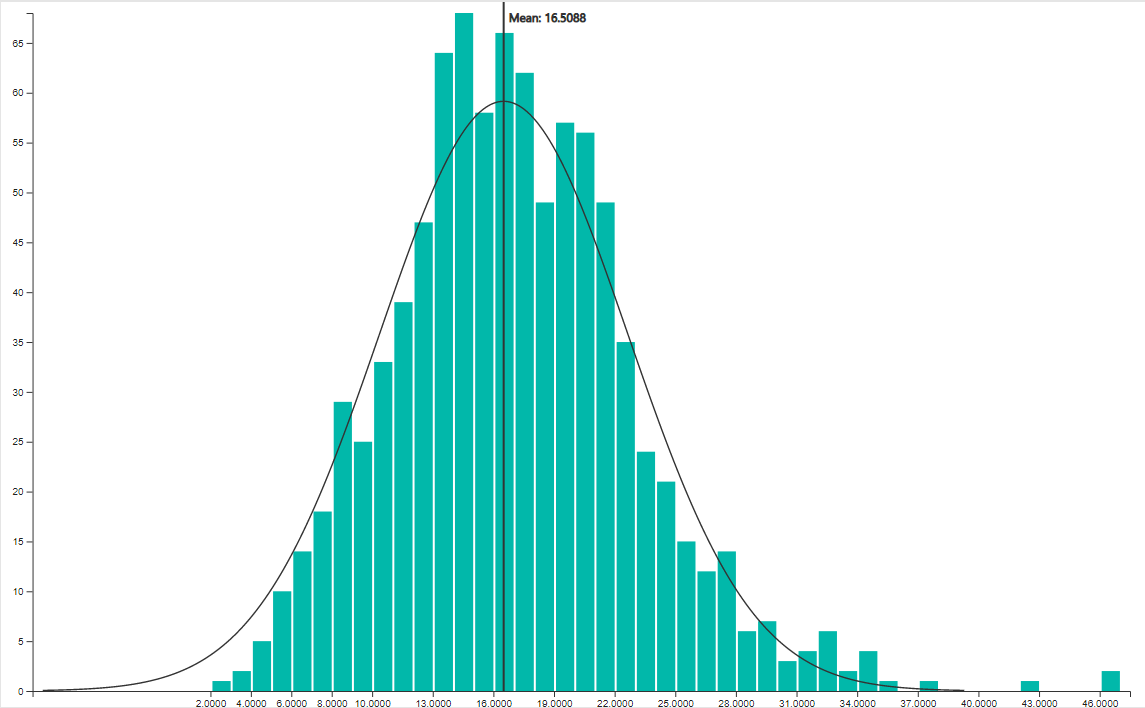
\includegraphics[width=0.75\textwidth]{assets/statistics/histogram.png}
    \caption{A histogram and the graph of the distribution of the samples}
\end{figure}

\begin{figure}[H]
    \centering
    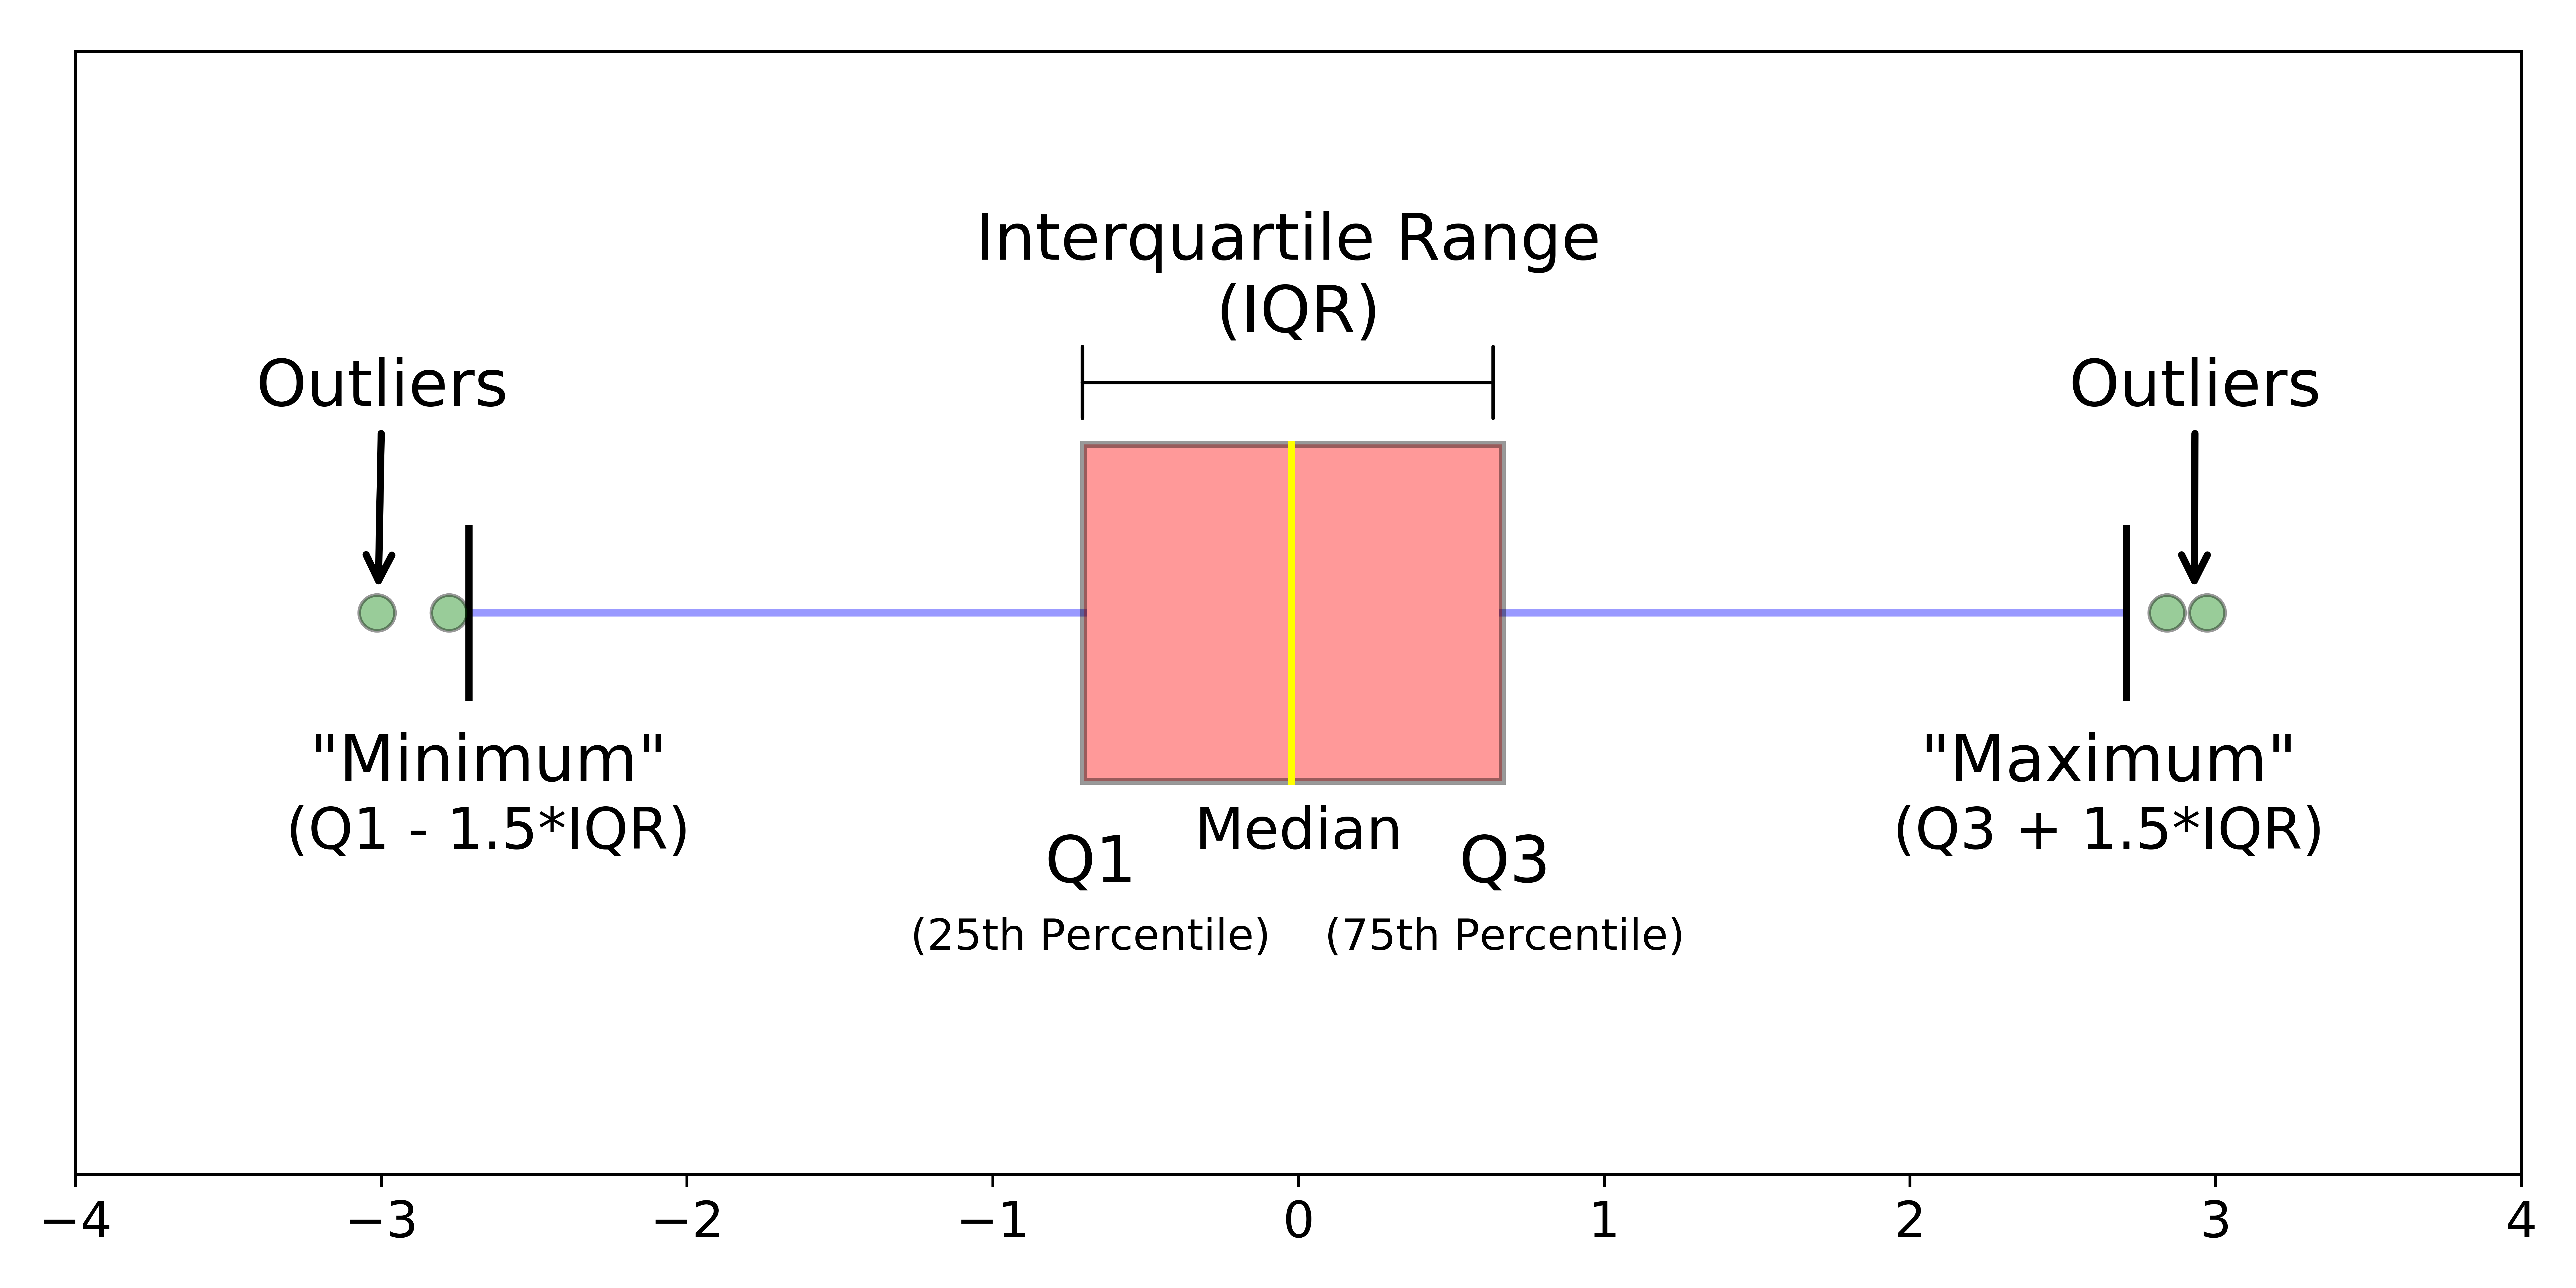
\includegraphics[width=0.75\textwidth]{assets/statistics/boxplot.png}
    \caption{A boxplot with indication on what the lines mean}
\end{figure}

Boxplots are very useful to check the symmetry of a sample.

\subsubsection{Location-Scale family of distributions}

\begin{definition}{Location-Scale family}{location-scale-family}
    Let $X$ be a random variable with distribution $F$ and $Y = a + bX$ with $b>0$.
    Then the distribution of $Y$ is
    \begin{equation}
        F_{a, b}(y) = F\left( \frac{y-a}{b} \right)
    \end{equation}
\end{definition}

\begin{example}{Normal distribution}{}
    $F$ is in the same location-scale family as the standard normal $\iff$ $F$ is a normal distribution
\end{example}

\subsubsection{Quantiles}

\begin{definition}{$\alpha$-quantiles}{alpha-quantiles}
    The $\alpha$-quantile of a distribution $F$ is given by
    \begin{equation}
        F^{-1}(\alpha) = \inf\{ x: F(x) \geq \alpha \}, \quad \alpha \in (0, 1)
    \end{equation}
\end{definition}

The quantile function of a location-scale family is
$F_{a, b}^{-1}(\alpha) = a + bF^{-1}(\alpha)$.

\begin{definition}{QQ-plot}{qq-plot}
    The QQ-plot for the realizations $x_1, \dots, x_n$ for a distribution function $F$ is a plot of the points
    \begin{equation}
        \left\{ \left( F^{-1}\left( \frac{i}{n+1} \right), x_i \right) : i = 1, \dots, n \right\}
    \end{equation}
    where $i$ is the order of the indices of $x_i$ such that they are in \textit{increasing order}.
\end{definition}

If the points $x_1, \dots, x_n$ come from $F$ then the points will approximately align to the $y = x$ line.
This is because we expect the sample quantile $x_i$ to be close to the theoretical quantile given by the formula.

\subsubsection{Correlation and independence}

As we know from Probability, we define the correlation coefficient as
\begin{equation}
    \rho_{A,B} = \frac{\cov(A, B)}{\sigma_A \sigma_B} \in [-1, 1]
\end{equation}

Recall that independence implies $\rho = 0$, but not viceversa (except for the normal distribution).

\begin{definition}{Sample correlation coefficient}{sample-correlation-coeff}
    Consider a sample of pairs $(X_1, Y_1), \dots, (X_n, Y_n)$.
    Then we define the sample correlation coefficient as
    \begin{equation}
        r_{X, Y} = \frac{\sum^n_{i = 1} (X_i - \bar{X})(Y_i - \bar{Y})}{(n-1)\sqrt{S^2_X} \sqrt{S^2_Y}}
    \end{equation}
\end{definition}

In the definition we use the following notation:
\begin{itemize}
    \item $\bar X$ is the sample mean
    \item $\sqrt{S^2_X}$ is the sample variance
\end{itemize}

We observe the following from $r_{X, Y}$:
\begin{itemize}
    \item $r_{X, Y} \in [-1, 1]$.
    \item If $r_{X, Y} = 1$ all the samples lie on the line $y = \bar y + \frac{S_y}{S_x}(x-\bar x)$.
    \item If $r_{X, Y} = -1$ all the samples lie on the line $y = \bar y - \frac{S_y}{S_x}(x-\bar x)$.
    \item If $X_1, \dots, X_n$ and $Y_1, \dots, Y_n$ are independent then $r_{X, Y}$ will be close to $0$.
\end{itemize}

Graphically we can observe correlation or independence using \textbf{scatter plots}: if the graph of $\{ (x_i, x_{i+1}) : i = 1, \dots, n-1 \}$ should show not much of a structure if the samples are independent.

\subsection{Estimation}

Estimation is the process of finding the best fitting distribution from the statistical model.

Suppose the model depends on an unknown parameter $\theta \in \Theta$:
\begin{equation}
    \mathcal M = \{ P_\theta : \theta \in \Theta \}
\end{equation}
Now we assume that $X = (X_1, \dots, X_n)$ has distribution $P_\theta$ for some $\theta \in \Theta$.
Then we want to find the $\theta$ that makes $P_\theta$ best fit the observed data.
We call this the \emph{true value of $\theta$}.
Sometimes it is even useful to compute the true value of some $g(\theta)$.

\begin{definition}{Estimator}{estimator}
    An \emph{estimator} is a random vector $T(X)$ that depends only on the observation $X$.

    The corresponding \emph{estimate} for a realization $x$ is $T(x)$.
\end{definition}

Note that estimators \emph{do not} depend on $\theta$.
The estimate will give us our value of $\theta$.

First, lets define some notation:
\begin{itemize}
    \item $T$ is the estimator $T(X)$.
    \item $t$ is the estimate $T(x)$.
    \item $\hat \theta$ is used for both the estimator and estimate of a unknown $\theta$ of interest
\end{itemize}

We could use as an estimator the distance between $T$ and $g(\theta)$
\begin{equation}
    \norm{T - g(\theta)}
\end{equation}

We want this difference to be as small as possible, that is, to be as concentrated as possible towards $0$.
Since $\norm{T - g(\theta)}$ is a random variable we can consider the one more concentrated around $0$.

\newcommand{\MSE}{{\operatorfont MSE}}

\begin{definition}{Mean squared error}{mean-squared-error}
    The mean squared error MSE of an estimator $T$ for the value of $g(\theta)$ is defined as
    \begin{equation}
        \MSE(\theta, T) = E_\theta\left(\norm{T - g(\theta)}^2\right)
    \end{equation}
    where $E_\theta$ is the expectation of $P_\theta$
\end{definition}

\begin{proposition}{MSE decomposition}{mse-decomposition}
    If a $T$ is real-valued estimator we can decompose the $\MSE$ as
    \begin{equation}
        \MSE(\theta, T) = V_\theta(T) + (E_\theta(T) - g(\theta))^2
    \end{equation}
\end{proposition}
\begin{proof}
    \begin{align}
        E_\theta\left((T - g(\theta))^2\right) & = E_\theta\left((T -E_\theta(T) + E_\theta(T) - g(\theta))^2\right)                                                            \\
                                               & = E_\theta(T-E_\theta(T))^2 - 2E_\theta(T-E_\theta(T))(E_\theta(T) - g(\theta)) + \cancel{E_\theta}(E_\theta(T) - g(\theta))^2 \\
                                               & = V_\theta(T) - 2 (E_\theta(T) - g(\theta)) \cancelto{0}{E_\theta(T-E_\theta(T))} - (E_\theta(T) - g(\theta))^2                \\
                                               & = V_\theta(T) - (E_\theta(T) - g(\theta))^2
    \end{align}
\end{proof}

We say that an estimator is \emph{biased} if it's expectation is not centered around $g(\theta)$.

\subsubsection{Maximum likelihood estimator}

\begin{definition}{Likelihood function}{likelihood-function}
    Let $X$ be a random vector with pdf $p_0$ that depends on a parameter $\theta \in \Theta$.
    For a fixed $x$ the likelihood function is defined as
    \begin{equation}
        \theta \mapsto L(\theta, x) = p_\theta(x)
    \end{equation}
\end{definition}

\begin{lemma}{IID variables}{}
    If $X_1, \dots, X_n$ IID then
    \begin{equation}
        L(\theta; X_1, \dots, X_n) = \prod_{i = 1}^{n} L(\theta, X_i)
    \end{equation}
\end{lemma}

\begin{definition}{Maximum likelihood estimator}{}
    The maximum likelihood estimate of $\theta$ is the value $T(x) \in \Theta$ that maximizes the likelihood function $L(\theta; x)$.

    The maximum likelihood estimator is $T(X)$.
\end{definition}

An useful trick we can use to find the maximum likelihood estimate is to apply the $\log$ to the likelihood function.
In this way we are left to deal with sums and not products (by the properties of logarithms), and, since $\log$ is monotone, the maximum of the transformation will be the maximum of the original function.

We will call \textbf{score function} the derivative of the likelihood function (or its log transformation).

The idea behind the likelihood function is that this is a function that, given an observation $x$, gives us the probability that the $\theta$ we chose was good.

\begin{example}{Exponential distribution}{mle-exponential}
    Let $X = (X_1, \dots, X_n)$ be a sample from the exponential distribution with unknown parameter $\lambda \in (0, \infty)$.
    Compute the MLE.
\end{example}

\begin{proof}[Solution]
    The sample space is
    \begin{equation}
        \mathcal{M} = \{ p_\lambda(x) = \lambda e^{-\lambda x}, x > 0 \}
    \end{equation}
    then we compute the pmf
    \begin{equation}
        p_\lambda (x_1, \dots, x_n) = \prod_{i = 1}^n (\lambda e^{-\lambda x}) = \lambda^n e^{-\lambda \sum_{i = 1}^n x_i}
    \end{equation}
    therefore, the likelihood function is
    \begin{equation}
        L(\lambda; x_1, \dots, x_n) = \lambda^n e^{-\lambda \sum_{i = 1}^n x_i}
    \end{equation}

    Now we want to maximize $L$ but it is easier to take the $\log$ first:
    \begin{equation}
        l(\lambda; x_1, \dots, x_n) = n\log(\lambda) + \lambda \sum_{i = 1}^n x_i
    \end{equation}
    and by differentiating we get the score equation to be
    \begin{equation}
        \frac{n}{\lambda} - \sum_{i = 1}^{n} x_i = 0
        \implies \hat \lambda = \frac{1}{\bar{x}}
    \end{equation}

    The last thing we are left to do is to make sure this is a maximum point, therefore we have to take the second derivative:
    \begin{equation}
        \dv{}{\lambda} \left( \frac{n}{\lambda} - \sum_{i = 1}^{n} x_i \right) = -\frac{n}{\lambda^2} < 0
    \end{equation}
    hence it is indeed a point of maximum.

    We conclude that $\hat \lambda = \frac{1}{\bar{x}}$ is the maximum likelihood estimate.
\end{proof}


\begin{example}{Coin tosses}{mle-bernoulli}
    A coin with unknown $p = P(\text{HEAD})$ is tossed $n = 100$ times and shows heads $60$ times.
    Compute the MLE.
\end{example}

\begin{proof}[Solution]
    Intuitively we would say that $p = 0.6$.
    Let's check it.

    We have that $X_1, \dots, X_n$ IID $\sim \Bernoulli(p)$ therefore
    \begin{align}
        L(p; X_1, \dots, X_n)         & = \prod_{i = 1}^n \left( p^{X_i} (1 - p)^{1-X_i} \right)   \\
                                      & = p ^{\sum_{i = 1}^n X_i} (1-p) ^{\sum_{i = 1}^n (1- X_i)} \\
                                      & = p^{n \bar X} (1-p)^{n(1-\bar{X})}                        \\
        l(p; X_1, \dots, X_n)         & = n \bar X \log p + n(1- \bar{X}) \log(1-p)                \\
        \dv{l(p; X_1, \dots, X_n)}{p} & = \frac{n \bar x}{p} - \frac{n(1-\bar{x})}{1-p}
    \end{align}

    Now we have our score function that we want to maximize:
    \begin{align}
        \max_p                           & \frac{n \bar x}{p} - \frac{n(1-\bar{X})}{1-p}                             \\
                                         & \implies \frac{\cancel {n} \bar X}{p} = \frac{\cancel{n}(1-\bar{X})}{1-p} \\
                                         & \implies \bar{X} (1-p) = p (1-\bar X)                                     \\
                                         & \implies \bar{X} -\cancel{p\bar{X}} = p -\cancel{p\bar{X}}
        \implies \hat p = \bar{X}                                                                                    \\
        \dv[2]{l(p; X_1, \dots, X_n)}{p} & = -\frac{n \bar{X}}{p^2} - \frac{n(1-\bar X)}{(1-p)^2} < 0                \\
                                         & \implies \hat p \text{ is the MLE.}
    \end{align}
    which indeed corresponds to the intuitive result.
\end{proof}

\begin{example}{Uniform distribution}{mle-uniform}
    Let $X_1, \dots, X_n \stackrel{\text{IID}}{\sim} \Uniform(0,\theta)$ with $\theta$ unknown.
    Compute the MLE.
\end{example}

\begin{proof}[Solution]
    \begin{align}
        L(\theta; X_1, \dots, X_n) & = \prod_{i = 1}^n \frac{1}{n} 1_{[0, \theta]}(x_i)                \\
                                   & =\theta^{-n} \prod_{i = 1}^n 1_{[x_i, \infty)} (\theta)           \\ % TODO: explain this better
                                   & = \theta^{-n} 1_{[x_1; \infty) \cap \dots \cap [x_n; \infty)}     \\
                                   & = \theta^{-n} 1_{\left[\max_n \{x_1, \dots, x_n\}; \infty\right)}
    \end{align}

    Now we can look at the two cases of the indicator function and we see that the maximum occurs at $\hat \theta = \max_n x_n$.
\end{proof}

\begin{example}{Normal distribution}{mle-normal}
    Let $X_1, \dots, X_n \stackrel{\text{IID}}{\sim} \Normal(\mu,\sigma^2)$ with $\mu,\sigma^2$ unknown.
    Compute the MLE.
\end{example}

\begin{proof}[Solution]
    \begin{align}
        L(\mu,\sigma^2; X_1, \dots, X_n)                   & = \prod_{i = 1}^n \frac{1}{\sqrt{2 \pi \sigma^2}} e^{-\frac{(X_i - \mu)^2}{2 \sigma^2}}                                 \\
                                                           & = (2 \pi \sigma^2)^{-\frac{n}{2}} e^{- \sum_{i = 1}^n \frac{(X_i - \mu)^2}{2 \sigma^2}}                                 \\
        l(\mu,\sigma^2; X_1, \dots, X_n)                   & = -\frac{n}{2}\log(2 \pi \sigma^2) - \sum_{i = 1}^n \frac{(X_i - \mu)^2}{2 \sigma^2}                                    \\
        \pdv{l(\mu,\sigma^2; X_1, \dots, X_n)}{\mu}        & = \cancel{-1 }\cdot \cancel{-} \sum_{i = 1}^n \frac{\cancel{2}(X_i - \mu)}{\cancel{2} \sigma^2}  \label{eq:mle-n-seq-1} \\
        \pdv{l(\mu,\sigma^2; X_1, \dots, X_n)}{(\sigma^2)} & = -\frac{n}{2 \sigma^2} + \sum_{i = 1}^n \frac{(X_i - \mu)^2}{2 \sigma^4} \label{eq:mle-n-seq-2}
    \end{align}

    Now we have that \cref{eq:mle-n-seq-1} and \cref{eq:mle-n-seq-2} are our score functions which we want to maximize.
    \begin{align}
        \sum_{i = 0}^{n} \frac{(X_i - \hat \mu)}{\sigma^2} = 0                      & \implies \hat \mu = \bar X                                            \\
        -\frac{n}{2 \sigma^2} + \sum_{i = 1}^n \frac{(X_i - \mu)^2}{2 \sigma^4} = 0 & \implies \hat{\sigma}^2 = \frac{1}{n} \sum_{i = 1}^n (X_1 - \bar X)^2
    \end{align}
    where we substituted the first result into the second equation in order to solve it.
    It can be shown that $\hat \mu$ and $\hat \sigma$ are maximizers but we'll omit it here.

    We see that $\hat \mu$ is unbiased while $\hat \sigma ^2$ is.
\end{proof}

\subsubsection{Method of moments estimators}

\begin{definition}{Moment and sample moment}{moment-sample-moment}
    Let $X \sim p_\theta$. The $j$-th moment of $X$ is given by
    \begin{equation}
        E_\theta(X^j),
    \end{equation}
    assuming the expectation exists.

    Similarly, the $j$-th sample moment of $X_1,\dots, X_n$ IID random variables is defined as
    \begin{equation}
        \bar{X_j} = \frac{1}{n} \sum_{i = 1}^n X_i^j \convas E_\theta(X^j)
    \end{equation}
    by the law of large numbers.
\end{definition}

The idea is that we compute the moment and the sample moment, then we choose the parameter such that the moment and the sample moment coincides.
This is very simple and most times it coincides with the MLE.
We repeat the process until the $k$-th moment, where $k$ is the smallest number such that the system has a unique solution.

\begin{example}{Common distributions}{}
    \begin{itemize}
        \item \emph{Exponential}: same result as MLE;
        \item \emph{Uniform}: $\hat \theta = 2 \bar X$ which is a worse result than the MLE.
    \end{itemize}
\end{example}

Note that in this way we are summarizing the distribution in $k$ values. A best method is to find the $\hat \theta$ that minimizes the distance between the two moments.
For example, if we use $l$ moments, we define the \emph{generalized method of moments} as
\begin{equation}
    \sum_{i = 0}^l \left( \frac{1}{n} \sum_{i = 0}^n X^j_i - E(X_i^j) \right)^2
\end{equation}
or, even more generally, for some fixed $g_1, \dots, g_n$,
\begin{equation}
    \sum_{i = 0}^l \left( \frac{1}{n} \sum_{i = 0}^n g_j(X_i) - E(g_j(X_i)) \right)^2
\end{equation}

\section{Bayesian statistics}

\label{sec:bayes}

\subsection{Introduction}

This is the oldest method of constructing estimators.
The main idea is that there is no unique true parameter, every parameter has it's own probability.
The main problem of this strategy is that there are problems with computing the result (except for simple cases).
Nowadays this method is widely used in combination with computer-based simulations.

\begin{definition}{Bayesian model}{bayesian-model}
    A statistical model in bayesian statistics is
    \begin{equation}
        \mathcal M = \{ p_\theta : \theta \in \Theta \}
    \end{equation}
    and a \emph{prior distribution} $\pi$ on the parameter space $\Theta$.
\end{definition}

Differently from before, $\theta$ is seen as a \emph{random variable}, not an unknown.
The choice of $\pi$ is driven by subjective belief, based on experience and likelihood of different values of $\theta$.
After observing the data we \emph{update our believes} by computing the posterior distribution.

\begin{definition}{Bayes risk}{bayes-risk}
    The Bayes risk of an estimator $T$ for a real-valued parameter $g(\theta)$ is defined as
    \begin{equation}
        R(\pi; T) = \int_\Theta E_\theta[(T-g(\theta)^2)] \pi(\theta) \dd{\theta}
    \end{equation}
\end{definition}
This is pretty much the equivalent of the MSE for bayesian models.

\begin{definition}{Bayes estimator}{bayes-estimator}
    The Bayes estimator with respect to the prior density $\pi$ is the estimator $T$ that minimizes $R(\pi; T)$.
\end{definition}

\begin{theorem}{Bayes estimator - first version}{bayes-estimator-v1}
    The Bayes estimator for $g(\theta)$ w.r.t. the prior density $\pi$ is
    \begin{equation}
        T(x) = \frac{\int_\Theta g(\theta) p_\theta(x)\pi(\theta) \dd{\theta}}{\int_\Theta g(\theta) \pi(\theta) \dd{\theta}}
    \end{equation}
\end{theorem}

\begin{proof}
    Start by the definition of bayesian risk and plug in the definition of expectation.
    \begin{align}
        R(\pi; T) & = \int_\Theta E_\theta[(T-g(\theta)^2)] \pi(\theta) \dd{\theta}                                               \\
                  & = \int_\Theta \left(\int_X (T-g(\theta))^2 p_\theta(x)\dd{x} \right) \pi(\theta) \dd{\theta}                  \\
                  & \stackrel{\text{fubini}}{=} \int_X \int_\Theta (T(x) - g(\theta))^2 p_\theta(x) \pi(\theta) \dd{\theta}\dd{x}
    \end{align}

    The goal is to minimize for all $x$. We can just minimize the inside integral as that will result in the minimization of the whole expression.
    \begin{align}
        \argmin & \int_\Theta (T(x) - g(\theta))^2 p_\theta(x) \pi(\theta) \dd{\theta}                                                                                                                    \\
                & = T^2(x) \int_\Theta p_\theta(x) \pi(\theta) \dd{\theta}- 2T(x) \int_\Theta g(\theta) p_\theta(x) \pi(\theta) \dd{\theta} + \int_\Theta g^2(\theta) p_\theta(x) \pi(\theta) \dd{\theta}
    \end{align}

    Now we take the derivative w.r.t. $T(x)$ and set it equal to zero:
    \begin{gather}
        \cancel 2 T(x) \int_\Theta p_\theta(x) \pi(\theta) \dd{\theta}- \cancel 2 \int_\Theta g(\theta) p_\theta(x) \pi(\theta) \dd{\theta} = 0 \\
        \implies T(x) = \frac{\int_\Theta p_\theta(x) \pi(\theta) \dd{\theta}}{\int_\Theta g(\theta) p_\theta(x) \pi(\theta) \dd{\theta}}
    \end{gather}
\end{proof}

\begin{definition}{Posterior distribution}{posterior-distribution}
    The posterior distribution of $\bar \Theta$ conditionally on $X = x$ is
    \begin{equation}
        p_{\bar \Theta | X = x} (\theta) = \frac{p_\theta(x) \pi(\theta)}{\int_\Theta p_\theta(x) \pi(\theta) \dd{\theta}}
    \end{equation}
\end{definition}

We say that the the prior and the posterior distribution are \emph{conjugated} if they belong to the same family of distributions.

Now we can rewrite \Cref{thm:bayes-estimator-v1} by substituting this new definition:

\begin{theorem}{Bayes estimator - second version}{bayes-estimator-v2}
    The Bayes estimator for $g(\theta)$ w.r.t. the prior density $\pi$ is
    \begin{equation}
        T(x) = \int_\Theta g(\theta) p_{\bar \Theta | X = x} (\theta) \dd{\theta} = E[g(\bar \Theta) | X = x]
    \end{equation}
\end{theorem}

\subsection{Estimation}

We can use an estimator $t = T(x)$ to estimate the value of $\theta$ but usually our estimate will be wrong, the point estimate $t$ will generally differ from $\theta$.
In this section we will try to quantify the difference between $t$ an $\theta$ and, if $\theta \in \R$, find an \emph{interval estimate} $[L(x), R(x)]$ where $\theta$ has a high probability of lying.

\begin{definition}{Confidence region}{confidence-region}
    Let $X$ be a random variable depending on a parameter $\theta \in \Theta$.
    Let $G_X \in \mathcal P(X)$.
    The map $X \mapsto G_X$ is a confidence region for $\theta$ of confidence level $1-\alpha$ if
    \begin{equation}
        P_\theta(G_X \ni \theta) \geq 1- \alpha \quad \forall \theta \in \Theta
    \end{equation}
    where usually $\alpha$ is small.
\end{definition}

We note the following facts:
\begin{enumerate}
    \item $G_X$ is a stochastic (i.e. random) subset of $\Theta$ as it depends on a random variable $X$; meanwhile $\theta$ is a fixed number.
    \item The event $\{ G_X \ni \theta \}$ has as random object $G_X$.
    \item Given a realization $X = x$, also $G_X$ realizes to $G_x$ which is therefore not random anymore.
    \item Since $G_x$ and $\theta$ are both fixed, then either $\theta \in G_x$ or $\theta \notin G_x$.
\end{enumerate}

In bayesian statistics we interpret the true value of $\theta$ as the realization of $\bar \Theta$.
In this context we can make a statement about the random parameter \emph{after} the realization $X = x$, of the type
\begin{equation}
    P(\bar \Theta \in G_X \mid X = x)
\end{equation}
and we can determine this probability by the posterior distribution of $p_{\bar \Theta \mid X = x}$.

If we focus on $\theta \in \R$ we have that confidence regions are usually intervals of the form $G_X = [R(X), L(X)]$.
If the interval is centered around the point estimate $t$ then it is called \emph{symmetric} and we write $\theta = t \pm \eta$ with $\eta = [R(x) - L(x)]/2$.

\begin{example}{Normal distribution}{}
    Let $X_1, \dots X_n$ be a sample from the normal distribution $\Normal(\theta, \sigma^2)$, with unknown mean $\theta$ and known variance $\sigma^2$.
    Find a confidence interval for $\theta$ of level of confidence $1-\alpha$.
\end{example}

\begin{proof}[Solution]
    We know that the MLE estimator for the normal is $\hat \theta = \bar X$.
    Let us now compute the expectation and variance of $\bar X$:
    \begin{align}
        E_{\theta} (\bar X) & = E_\theta \left( \oneover{n} \sum_{i = 1}^n X_i \right) = \oneover n \sum_{i = 1}^n E_\theta(X_i) = \theta                \\
        V_{\theta} (\bar X) & = V_\theta \left( \oneover{n} \sum_{i = 1}^n X_i \right) = \oneover{n^2} \sum_{i = 1}^n V_\theta(X_i) = \frac{\sigma^2}{n}
    \end{align}

    From these result we can write $\bar X$ as the rescaling of a standard gaussian $Z$:
    \begin{equation}
        \bar X = \frac{\sigma}{\sqrt{n}} Z + \theta
    \end{equation}

    We define the $\alpha$-quantile of a standard gaussian as $\xi_\alpha$ (as in \Cref{def:alpha-quantiles}).
    This means that
    \begin{align}
        \alpha                                                 & = P(Z \leq \xi_\alpha) \implies                                        \\
        P(\xi_{\alpha/2} \leq Z \leq \xi_{1-\frac{\alpha}{2}}) & = P(Z \leq \xi_{1-\frac{\alpha}{2}}) -P(Z \leq \xi_{\frac{\alpha}{2}}) \\
                                                               & = 1-\frac{\alpha}{2} -\frac{\alpha}{2} = 1- \alpha
    \end{align}
    So now we can compute the confidence interval by substituting $Z$ with our rescaling of $\bar X$:
    \begin{align}
        1 - \alpha & = P(\xi_{\alpha/2} \leq Z \leq \xi_{1-\frac{\alpha}{2}})                                                                                 \\
                   & = P\left(\xi_{\alpha/2} \leq \frac{\bar X - \theta}{\sigma / \sqrt n} \leq \xi_{1-\frac{\alpha}{2}}\right)                               \\
                   & = P\left(\frac{\sigma}{\sqrt n}\xi_{\alpha/2} - \bar X \leq - \theta \leq \frac{\sigma}{\sqrt n}\xi_{1-\frac{\alpha}{2}} - \bar X\right) \\
                   & = P\left(\bar X - \frac{\sigma}{\sqrt n}\xi_{\alpha/2} \geq \theta \geq \bar X -\frac{\sigma}{\sqrt n}\xi_{1-\frac{\alpha}{2}}\right)    \\
                   & = P\left(\bar X + \frac{\sigma}{\sqrt n}\xi_{1-\alpha/2} \geq \theta \geq \bar X -\frac{\sigma}{\sqrt n}\xi_{1-\frac{\alpha}{2}}\right)
    \end{align}
    which gives us a confidence interval of
    \begin{equation}
        \bar X \pm \frac{\sigma}{\sqrt n}\xi_{1-\alpha/2} = [\bar X - \frac{\sigma}{\sqrt n}\xi_{1-\alpha/2}, \bar X - \frac{\sigma}{\sqrt n}\xi_{1-\alpha/2}]
    \end{equation}
\end{proof}

\subsection{Pivots}

\begin{definition}{Pivot}{pivot}
    A pivot is a function $T(X, \theta)$ whose probability distribution does not depend on $\theta$ or any other parameter.
\end{definition}

Note that for a pivot $T(X, \theta)$ the probability $P_\theta(T(X, \theta) \in B)$ is not a function of $\theta$.

For the normal distribution a pivot is
\begin{equation}
    T(X, \theta) = \frac{\bar X - \theta}{\sigma /\sqrt{n}}
\end{equation}
which is distributed according to the standard normal.

We can define a confidence region for a pivot as well.
For every $B$ such that $P_\theta(T(X, \theta) \in B) \geq 1- \alpha$, the set
\begin{equation}
    \{ \theta \in \Theta : T(X, \theta) \in B \}
\end{equation}
is the confidence region for $\theta$ of confidence level $1- \alpha$.

\begin{example}{Uniform distribution}{}
    Let $X_1,...,X_n$ be a sample from the uniform distribution $\Uniform(0,\theta)$, with $\theta$ unknown.
    Find a confidence interval for $\theta$ of level of confidence $1 - \alpha$.
\end{example}

\begin{proof}[Solution]
    We notice that while $X_i \sim \Uniform(0, \theta)$, if we rescale we get $X_i/ \theta \sim \Uniform(0,1)$.
    As the MLE for the uniform distribution is $X_{(n)}$ (the maximum observation of $X$), the MLE of our rescaled version is $X_{(n)} / \theta$.
    We can prove (even if it is quite obvious in this case) that
    \begin{equation}
        T(X; \theta) = X_{(n)} / \theta
    \end{equation}
    is a pivot as its distribution is independent from $\theta$.

    Now we can find the confidence interval.
    We have to choose some $c, d$ s.t $[c, d] \subseteq [0, 1]$ and the following holds:
    \begin{equation}
        1 - \alpha =  P(c \leq T(X; \theta) \leq d) = P (T(X, \theta) \leq d) - P (T(X, \theta) \leq c) = d^n - c^n
    \end{equation}
    that is
    \begin{align}
        c = 0 & \implies d = (1- \alpha)^{\frac{1}{n}} \\
        d = 0 & \implies c = \alpha^{\frac{1}{n}}
    \end{align}

    Then the confidence region can be calculated by
    \begin{align}
        1 - \alpha         & = P\left(c \leq \frac{X_{(n)}}{\theta} \leq d\right)                  \\
                           & = P\left(\frac{X_{(n)}}{c} \geq \theta \geq \frac{X_{(n)}}{d} \right) \\
        \implies \text{CI} & = \left[ \frac{X_{(n)}}{d}, \frac{X_{(n)}}{c} \right]
    \end{align}
\end{proof}

\subsubsection{Near-pivot}

While pivots are definitely useful there is not always possible to find one.
The solution to this problem is to find a function $T(X; \theta)$ whose distribution can be approximated by a distribution that does not depend on $\theta$.
We call this function \textbf{near-pivot} and it typically available when we deal with large samples and therefore we are able to use limit theorems (like the central limit theorem).

More precisely an estimator $T_n = T_n(X)$ is a near pivot if it satisfies
\begin{equation}
    \frac{T_n - g(\theta)}{\sigma_{n, \theta}} \convdist \Normal(0,1)
\end{equation}
or, equivalently
\begin{equation}
    \lim_{n \to \infty} P_\theta \left( \frac{T_n - g(\theta)}{\sigma_{n, \theta}} \leq x \right) = \Phi(x) \quad \forall x
\end{equation}
where the standard deviation $\sigma_{n, \theta}$ of $T_n$ is often estimated by $\hat \sigma_n$ called the \emph{standard error}.
Then the approximate symmetric confidence level is
\begin{equation}
    g(\theta) \in T_n \pm \hat \sigma_n \xi_{1-\frac{\alpha}{2}}
\end{equation}

Moreover, an important near-pivot is the MLE which, under certain conditions, we claim it is asymptotically normal.

\subsubsection{Fisher information}

Let the observation $X_1$ have distribution $p_\theta$.
We know that the score function is defined as
\begin{equation}
    \dot \ell_\theta (x) = \pdv{}{\theta} \log p_\theta(x)
\end{equation}

\begin{definition}{Fischer information}{fischer-information}
    \begin{equation}
        i_\theta = V_\theta \left(\dot \ell_\theta (X_1)\right)
    \end{equation}
\end{definition}

\begin{proposition}{Properties of Fisher information}{props-fisher}
    If $\ell_\theta(x) = \log p_\theta(x)$ is twice differentiable for all $x$, under certain regularity conditions we have
    \begin{enumerate}[label=\roman*.]
        \item $E_\theta \ell_\theta (X_1) = 0$
        \item $i_\theta = -E_\theta \ddot\ell_\theta(X_1)$
    \end{enumerate}
\end{proposition}

\begin{proof}
    TODO: see lecture notes of CL10
\end{proof}

\begin{theorem}{Asymptotic normality of the MLE}{asymptotic-normality-mle}
    Let $\hat \theta_n$ be the ML estimator for $\theta$ based on a sample of size $n$ IID according to $p_\theta$.
    Under some regularity assumptions the sequence $\sqrt n (\hat \theta_n - \theta)$ converges in distribution to a normal distribution with expectation $0$ and variance $i_\theta^{-1}$, that is
    \begin{equation}
        \sqrt n (\hat \theta - \theta) \convdist \Normal(0, i_\theta^{-1})
    \end{equation}
    which means that
    \begin{equation}
        \sqrt{n i_\theta}(\hat \theta - \theta) \convdist \Normal(0, 1)
    \end{equation}
\end{theorem}

\subsubsection{Wald interval}

The problem is that we don't know $i_\theta$, but we can estimate it:
\begin{itemize}
    \item The \emph{plug-in estimator} for $i_\theta$ is $\hat i_\theta = i_{\hat \theta}$.
    \item The \emph{observed information} estimator, recalling that $E_\theta \ell_\theta (X_1) = 0$,
          \begin{equation}
              \hat i_\theta = -\oneover{n} \sum_{i = 1}{n} \ddot \ell_{\hat \theta}
          \end{equation}
\end{itemize}

The consequence is that we can consider a \emph{normal approximate} $(1-\alpha)$-confidence interval for $\theta$:
\begin{equation}
    \theta = \hat \theta_n \pm \oneover{\sqrt{n \hat i_\theta}} \xi_{1- \frac{\alpha}{2}}
\end{equation}
We call this interval \textbf{Wald interval}.

\subsubsection{Bootstrap}

We observe $x_1, \dots, x_n$, construct a statistical model and choose an estimator $\hat \theta$.
Now generate a new dataset from $p_{\hat\theta}$ of the same size $n$ as the original data.
Using the new realizations $x_1^*, \dots, x_n^*$ we estimate again with $\hat \theta^*$.
Repeat these steps a big number of times $\beta$ and we will get $\hat \theta_1, \dots, \hat \theta_\beta$ which can be seen as the realizations of the same estimator $\hat \theta$.
Then we can estimate the variance of $\hat \theta$ as
\begin{equation}
    \hat \sigma_{\beta}^2 = \sum_{i = 1}^\beta \frac{(\hat \theta_i^* - \hat \theta)^2}{\beta}
\end{equation}
and we can use as confidence interval
\begin{equation}
    \hat \theta \pm \xi_{1 - \alpha/2} \hat \sigma_\beta
\end{equation}

\subsubsection{Extra notions}

In lecture notes CL10 you can find the so called \say{regularity assumptions} introduced in the proof above, the extension to the multidimensional case, and the Bernstein-von Mises theorem.
These topics are not required for the exam.

\section{Hypothesis testing}

Statistics is used to \say{prove} hypothesis in sciences, where we just have data with measurement error.
Do we have enough evidence to say that the some new therapy is better than the old one?

We start with a statistical model for some observations.
The two hypothesis are coded in sets of parameters $\Theta_0, \Theta_1$ a partition of $\Theta$, such that if $\theta \in \Theta_0$ corresponds to the \textbf{null hypothesis} and if $\theta \in \Theta_1$ it corresponds to the \textbf{alternative hypothesis}.

Our goal is to determine if the alternative hypothesis $H_1$ is valid or not.
If $H_1$ is valid, we discard the null hypothesis $H_0$, or, if we do not have enough evidence, we cannot discard $H_0$ which means we cannot accept $H_1$ to be correct.

We can make two types of mistakes while doing this estimation:
\begin{itemize}
    \item Type I errors mean we reject $H_0$ even if it is correct (very bad)
    \item Type II errors mean we do not reject $H_0$ when it is incorrect (less bad)
\end{itemize}

\begin{definition}{Statistical test}{statistical-test}
    Given $H_0$, a statistical test consists of a set $K$ of possible values for the observations of $X$ called the \textbf{critical region}.
    Given an observation $x$, if $x \in K$ we \emph{reject} $H_0$, while if $x \notin K$ we \emph{do not reject} $H_0$.
\end{definition}

When we have $X = (X_1, \dots, X_n)$ it is generally useful to choose a test statistic $T$ that we deem appropriate and define the critical region as
\begin{equation}
    K = \{ (x_1, \dots, x_n) : T(x) \in K_T \}
\end{equation}
for some suitable $K_T$ (which is also called critical region).

Many times the critical region takes the form of
\begin{align}
    K_T & = \{ T \geq c_{\alpha_0} \}                                \\
    K_T & = \{ T \leq c_{\alpha_0} \}                                \\
    K_T & = \{ T \leq c_{\alpha_0} \} \cap \{ T \geq d_{\alpha_0} \}
\end{align}
where $c_{\alpha_0}$ is a number that we need to identify.

We now have to find a way of choosing $K$.
First, we can measure the quality of a test with the \textbf{power function}.
\begin{equation}
    \theta \mapsto \pi(\theta; K) = P_\theta(X \in K)
\end{equation}
the goal is to choose $K$ such that $\pi(\theta, K)$ is close to $0$ when $\theta \in \Theta_0$ and close to $1$ when $\theta \in \Theta_1$.

\begin{definition}{Size of a test}{size-of-test}
    The size of a critical region is the number
    \begin{equation}
        \alpha = \sup_{\theta \in \Theta_0} \pi(\theta; K)
    \end{equation}

    A test has \textbf{significance level} $\alpha_0$ if $\alpha \leq \alpha_0$.
\end{definition}

By choosing a significance level $\alpha_0$ we ensure that the probability of a type I error is at most $\alpha_0$.
We would like $\alpha_0$ to be small, but we cannot make it too small otherwise we would have an extremely small $K$ and the probability of a type II error becomes higher.
Usually a good choice for $\alpha_0$ is $0.05$.

Usually we will fix $\alpha_0$ and, between two tests, we will choose the one with higher $\alpha$ (therefore with smaller probability of type II error).

Once we find $\alpha_0$ we can also find $c_{\alpha_0}$ and viceversa.
In fact $c_{\alpha_0}$ is the smallest value for which the corresponding test has size smaller or equal to $\alpha_0$:
\begin{equation}
    c_{\alpha_a} = \min \left\{ t : \sup_{\theta \in \Theta_0} P_\theta (T(X)\geq t) \leq \alpha_0 \right\}
    \label{eq:def-c0}
\end{equation}

\subsection{One-sided and two-sided hypothesis tests}

We say that the hypothesis is \textbf{one-sided} if either
\begin{equation}
    H_0 = \{\theta : \theta \leq \theta_0\} \quad \text{or} \quad H_0 = \{\theta : \theta \geq \theta_0\}
\end{equation}
where the first case is called \emph{right one-sided} and the second one is \emph{right two-sided}.

We say that the hypothesis is \textbf{two-sided} if
\begin{equation}
    H_0 = \{ \theta: \theta = \theta_0 \} \implies H_1 = \{ \theta : \theta \ne \theta_0 \}
\end{equation}

\subsection{\texorpdfstring{$p$}{p}-values}

$p$-values are another way of describing a test.
By now we have seen critical regions and test-statistics but we can use $p$-values as well: these methods are equivalent.

Recall \Cref{eq:def-c0}: in that case we rejected $H_0$ if $t = T(x) \geq c_{\alpha_0}$ which is equivalent to
\begin{equation}
    t \geq c_{\alpha_a} \iff \underbrace{\sup_{\theta \in \Theta_0} P_\theta (T(X)\geq t)}_{p\text{-value}} \leq \alpha_0
\end{equation}

\begin{definition}{$p$-value (for right-sided critical regions)}{p-value-right}
    Consider a right-sided critical region $K_T$.
    Let $t$ be the observation of the test statistic $T$.
    Then the $p$-value is defined as
    \begin{equation}
        \sup_{\theta \in \Theta_0} P_\theta(T \geq t)
    \end{equation}
\end{definition}

Then the test becomes
\begin{itemize}
    \item $p$-value $\leq \alpha_0 \implies$ reject $H_0$
    \item $p$-value $> \alpha_0 \implies$ retain $H_0$
\end{itemize}

Equivalently we can define $p$-values for left-sided and double-sided critical regions:
\begin{gather}
    \sup_{\theta \in \Theta_0} P_\theta (T {\color{red} \leq} t)\\
    {\color{red} 2 \min }\left( \sup_{\theta \in \Theta_0} P_\theta (T \geq t), \sup_{\theta \in \Theta_0} P_\theta (T \leq t) \right)
\end{gather}
or in general, the smallest value of $\alpha$ for which the corresponding test rejects $H_0$.

\section{Tests}

\subsection{Binomial test}

TODO

\subsection{Gauss test (\texorpdfstring{$z$}{z}-test)}

Assume we have $X_1, \dots, X_n \stackrel{\text{IID}}{\sim} \Normal(\theta, \sigma^2)$, where $\sigma^2$ is known.
Consider $H_0 = \{ \theta \leq \theta_0 \}$ and $H_1 = \{ \theta \gt \theta_0 \}$ (right one-sided).

Lets choose the estimator to be the sample mean (which happens to be the MLE for the normal): $T(X) = \bar X$.

We can do better though: we can rescale $T$ to get
\begin{equation}
    \tilde{T}(X) = \frac{\bar X - \theta_0}{\sigma /\sqrt{n}} \sim \Normal\left(\sqrt{n} \frac{\theta - \theta_0}{\sigma}, 1\right)
\end{equation}
such that if $\theta = \theta_0$ we get $\Normal(0,1)$.

Choose $K_{\tilde T} = [ \tilde c_\alpha, \infty )$ and impose that $\alpha_0 \geq \alpha$ so
\begin{equation}
    \sup_{\theta \in \Theta_0} \pi(\theta, L) = \sup_{\substack{\theta \in \Theta_0 \\ \theta \leq \theta_0}} P_\theta (\tilde T \geq \tilde c_{\alpha_0}) = P_{\theta_0}(\tilde T \geq c_{\alpha_0})
\end{equation}
which is especially nice because now $\tilde T$ is distributed according to $\Normal(0,1)$.
\begin{gather}
    \alpha_0 \geq 1- \Phi(c_{\alpha_0}) \\
    c_{\alpha_0} \geq \Phi^{-1}(1- \alpha_0) = \xi_{1-\alpha_0}
\end{gather}
which means that all critical regions $K_{\tilde T} = [c; \infty)$ are admissible, with $c \geq \xi_{1 - \alpha_0}$.
Among these regions we choose the one which is most powerful, which we know already is $K_{\tilde T} = [\xi_{1-\alpha_0}, \infty)$.

Now we can choose some $\beta$ such that the type II error is bounded by it (for example max $10\%$).
We now want to compute how many people we need to interview to get the type II error below $\beta$ at a given $\theta^*$, where $\theta^*$ is a \say{guess} of a likely value of $\theta$.
\begin{equation}
    \beta \geq P_{\theta^*}(\text{type II error}) = P_{\theta^*}(\tilde T \notin K_{\tilde T}) = P_{\theta^*}(\tilde T \leq \xi_{1-\alpha_0})
\end{equation}
We now have to solve for $n$.
\begin{align}
    \beta                          & \geq P_{\theta^*}\left(\frac{\bar X - \theta_0}{\sigma / \sqrt n} \leq \xi_{1-\alpha_0}\right)                                              \\
                                   & = P_{\theta^*}\left(\frac{\bar X - \theta^*}{\sigma / \sqrt n} \leq \xi_{1-\alpha_0}  - \frac{\theta^* - \theta_0}{\sigma / \sqrt n}\right) \\
                                   & = P_{\theta^*}\left(Z \leq \xi_{1-\alpha_0}  - \frac{\theta^* - \theta_0}{\sigma / \sqrt n}\right)                                          \\
                                   & = \Phi\left(\xi_{1-\alpha_0}  - \frac{\theta^* - \theta_0}{\sigma / \sqrt n}\right)                                                         \\
                                   & = \Phi\left(\xi_{1-\alpha_0}  - (\theta^* - \theta_0) \frac{\sqrt n}{\sigma}\right)                                                         \\
    \implies \Phi^{-1}(\beta)      & \geq \xi_{1-\alpha_0}  - (\theta^* - \theta_0) \frac{\sqrt n}{\sigma}                                                                       \\
    \xi_{1-\alpha_0} - \xi_{\beta} & \geq (\theta^* - \theta_0) \frac{\sqrt n}{\sigma}                                                                                           \\
    n                              & \geq \sigma^2 \left(\frac{\xi_{1-\alpha_0} - \xi_{\beta}}{\theta^* - \theta_0}\right)^2
\end{align}
we had to introduce the shift because before it was centered around $\theta_0$, while we want it to be centered around $\theta^*$.

This procedure works also for left one-sided and two-sided hypothesis.

\subsection{\texorpdfstring{$t$}{t}-test}

So far we have covered samples from the normal distribution only when the variance was known.
To deal with the cases where the variance is also unknown we have to introduce the \emph{Student} distribution.

\begin{definition}{Student distribution}{strudent-}
    A random variable $T$ has Student distribution with $n$ degrees of freedom, denoted by $t_n$, if $T$ has the same distribution as
    \begin{equation}
        \frac{Z}{\sqrt{(\sum^n_{i=1} Z_i^2)/n}}
    \end{equation}
    where all the $Z$ are independent and distributed according to $\Normal(0,1)$.
\end{definition}

\begin{theorem}{Properties of normal samples}{prop-normal-samples}
    If $X_1, \dots, X_n$ are samples from $\Normal(\mu, \sigma^2)$, then:
    \begin{enumerate}[label=\roman*.]
        \item $\bar X \sim \Normal(\mu, \sigma^2/n)$
        \item $(n-1)\frac{S_X^2}{\sigma^2} \sim \mathcal X^2_{n-1}$, where $\mathcal X$ is Chi distributed
        \item $\bar X \indep S_X^2$
        \item $\sqrt n \frac{\bar X - \mu}{S_X} \sim t_{n-1}$
    \end{enumerate}
\end{theorem}

TODO: complete here

\subsection{Two samples tests}

In this case we have two samples
$X_1, \dots, X_n \stackrel{\text{IID}}{\sim}P_X$ and
$Y_1, \dots, Y_n \stackrel{\text{IID}}{\sim}P_Y$.
We want to compare $P_X$ and $P_Y$.

Our sample can be of two forms:
\begin{itemize}
    \item \emph{Paired observations}
          \begin{equation}
              (X_1, Y_1), \dots, (X_n, Y_n) \stackrel{\text{IID}}{\sim} P_{(X, Y)}
          \end{equation}
    \item \emph{Independent observations} (check independence of the samples)
          \begin{equation}
              X_1, \dots, X_n \indep Y_1, \dots, Y_m
          \end{equation}
\end{itemize}

\subsubsection{T-test for paired observations}

Let $Z_i = X_i - Y_i$ and $\Delta = \mathbb E Z_i$.
We want to check if $\Delta = 0$ or not.
We will assume that $Z_i \sim \Normal(\Delta, \sigma^2)$.

If $X_i \sim \Normal(\mu, \sigma_X^2)$ independent from $Y_i \sim \Normal(\mu - \Delta, \sigma_Y^2)$
we get that $Z_i \sim \Normal(\Delta, \sigma_X^2 + \sigma_Y^2)$.

We can also have that $X_i$ and $Y_i$ are not independent.
This is actually better, because this gives us a smaller variance, thus a better test.
This result comes from the formula
\begin{equation}
    V(Z_i) = V(X_i) + V(Y_i) - 2 \cov (X_i, Y_i)
\end{equation}

Once we have the hypothesis we just use the $t$-test on $Z_i$.

\subsubsection{Two-sample T-test}

In this case $X_i \sim \Normal(\mu, \sigma^2)$ and $Y_i \sim \Normal(\nu, \sigma^2)$
with the same variance.

Our hypothesis are $H_0 : \mu - \nu \leq 0$ and $H_1 : \mu - \nu > 0$.
We use the sample mean as test: $\bar X- \bar Y$ os gaussian with mean $\mu - \nu$
and variance $\sigma^2 \left(\oneover m + \oneover n\right)$.

Note that we don't have the variance, however we can estimate it as the weighted average of the sample variances
\begin{equation}
    S^2_{X, Y} = \frac{\sum^m_{i = 1} (X_i - \bar X)^2 + \sum^n_{i = 1} (Y_i - \bar Y)^2 }{n + m - 2}
\end{equation}

We get that $T$ is student distributed with $m + n - 2$ degrees of freedom:
\begin{equation}
    T = \frac{\bar X - \bar Y - 0}{S_{X, Y} \sqrt{\oneover m + \oneover n}}
\end{equation}
and from here proceed as in the normal $t$-test.

\subsubsection{Asymptotic T-test}

If we are in the same situation as the two-sample $t$-test but we have different variances
we cannot proceed as usual as it would encounter bad results.
However, if we have a large number of samples we can use limit theorems in order to get a better approximation.

Consider as test statistic
\begin{equation}
    T = \frac{\bar X - \bar Y}{\sqrt{\frac{S_X^2}{m} - \frac{S_Y^2}{n}}}
\end{equation}
and if our $H_0$ is defined as $H_0 : \mu \leq \nu$
we can consider an approximate critical region of $(\xi_{1-\alpha_0}, \infty)$.

% TODO: wilcoxon, goodness of fit, likelihood

\section{Optimality Theorem}

In this section we will try to find the \say{best} estimator and test.
The first step in this process is to remove the unneeded data.

\subsection{Sufficient statistic}

We want to find a summary statistic $V(X)$ of $X = (X_1, \dots, X_n)$ containing all the relevant information of $X$.

\begin{definition}{Sufficient statistic}{sufficient-statistic}
    Let $X$ be a statistical model of discrete probability distributions that depend on a parameter $\theta$.
    A statistic $V = V(X)$ is called sufficient if
    \begin{equation}
        P(X = x \mid V = v) \text{ does not depend on } \theta
    \end{equation}
\end{definition}

\begin{example}{Bernoulli}{}
    Consider a model $X_1, \dots, X_n \sim \Bernoulli(p)$.
    Prove that the statistic
    \begin{equation}
        V(X) = \sum_{i =1}^n X_i \sim \Binomial(n, p)
    \end{equation}
    is a sufficient statistic.
\end{example}

\begin{proof}
    \begin{align}
        P(X = x \mid V = v) & = \frac{X = x, V = v}{V = v}                                                                          \\
                            & = \frac{\prod P(X_i = x_i)}{P(V = v)}                                                                 \\
                            & = \frac{\cancel{p^{\sum x_i}} \cancel{(1-p)^{n - \sum x_i}}}{\binom{n}{v} \cancel{p^v (1-p)^{n - v}}}
    \end{align}
\end{proof}

\begin{theorem}{Factorization theorem}{factorization}
    Suppose that the statistical model for $X$ consists of discrete distributions.
    A statistic $V = V(X)$ is sufficient if and only if there exists $v \mapsto g_\theta(v)$ and $x \mapsto h(x)$
    such that for all $x$ and $\theta$
    \begin{equation}
        p_\theta(x) = g_\theta (V(x)) h(x)
    \end{equation}
    where $p_\theta$ is the probability mass function of $X$.
\end{theorem}

\begin{proof}
    First assume that $V$ is a sufficient statistic:
    \begin{align}
        p_\theta(X = x) & = p_\theta(X = x, V = v)                                                                               \\
                        & = \underbrace{p_{\cancel{\theta}}(X = x \mid V = v)}_{h(x)} \underbrace{p_\theta(V = v)}_{g_\theta(v)}
    \end{align}

    Now suppose that $p_\theta$ is factorizable:
    \begin{align}
        p_\theta(X = x_0 \mid V = v) & = \frac{p_\theta(X = x_0, \cancel{V = v})}{p_\theta(V = v)}                        \\
                                     & = \frac{p_\theta (X = x_0)}{\sum_{x: V(x) = v} p_\theta (X = x)}                   \\
                                     & = \frac{g_\theta(V(x_0)) h(x_0)}{\sum_{x: V(x) = v} g_\theta(V(x)) h(x)}           \\
                                     & = \frac{\cancel{g_\theta(v)} h(x_0)}{\cancel{g_\theta(v)} \sum_{x: V(x) = v} h(x)}
    \end{align}
    which indeed does not depend on $\theta$.
\end{proof}

Note that sufficient statistics are \emph{not unique}.
Our goal is to find one that is simple.

\begin{lemma}{}{}
    Let $V$ be a sufficient statistic and $f$ be a one-to-one map.
    Then $V = f(V^*)$ is sufficient if and only if $V^*$ is also sufficient.
\end{lemma}

For example, we can show that for a gaussian distributed sample,
a minimal statistic depends only on $\bar X$ and $S_X^2$.

Similarly, for a uniform distributed sample $X_{(n)}$ (the largest sample) is a sufficient statistic.

\subsection{Optimality theory}

We want to find the best estimator, which gives us the smallest MSE.
But this is impossible, because $T(X) = g(\theta_0)$ has 0 MSE everywhere, which is impossible.
Therefore we have to relax our requirements:
\begin{itemize}
    \item The \emph{Bayes criterion} (\Cref{sec:bayes}) minimizes the weighted average MSE.
          \begin{equation}
              \int \MSE(g(\theta), T) \pi(\theta) \dd \theta
          \end{equation}
    \item The \emph{Minmax criterion} minimizes the worst case scenario MSE:
          \begin{equation}
              \sup_{\theta \in \Theta} \MSE(T(x), g(\theta))
          \end{equation}
    \item \emph{Universal Minimum Variance Unbiased estimator} (UMVU) is an estimator for $g(\theta)$
          which is unbiased and has a smaller variance than any other estimator.
          Note that it is not always possible to find one.
\end{itemize}

\subsubsection{Constricting UMVU estimators}

\begin{theorem}{Rao-Blackwell}{rao-blackwell}
    Let $V$ be a sufficient statistic and $T$ a real valued estimator for $g(\theta)$.
    Then there exists an estimator $T^*(V)$ for $g(\theta)$ which depends only on $V$ such that
    $E_\theta T = E_\theta T^*$ and var$_\theta T^* \leq$ var$_\theta T$ for all $\theta$.
    In particular $\MSE(T, g(\theta)) \geq \MSE(T^*, g(\theta))$.
\end{theorem}

\begin{proof}
    Let us consider only discrete cases.

    Let $T^* = E(T\mid V)$ which by definition does not depend on $\theta$, then $T^*$ is an estimator.
    We have
    \begin{equation}
        E_\theta T^* = \sum_V T^* (v) p_\theta(V = v) = \sum_V E(T(V = v) p_\theta(V = v)) = E_\theta T
    \end{equation}

    Furthermore,
    \begin{align}
        E_\theta T T^* & = \sum_V E_\theta(T T^*) p_\theta(V = v)                \\
                       & = \sum_V T^*(v) E_\theta(T \mid V = v) p_\theta (V = v) \\
                       & = \sum_V T^*(v)^2 p_\theta(V = v) = (ET^*)^2
    \end{align}
    which gives us
    \begin{equation}
        \var_\theta (T) = \E_\theta T^2 - (\E_\theta(T))^2 \geq \E_\theta (T^*)^2
    \end{equation}

    TODO: explain this better, can be asked during the exam
\end{proof}

\begin{definition}{Complete statistic}{complete-statistic}
    A statistic $V$ is complete if $\E_\theta f(V) = 0$ for all $\theta \in \Theta$
    holds only for functions $f$ such that
    \begin{equation}
        p_\theta(f(V) = 0) = 1
    \end{equation}
\end{definition}

This definition means that it is impossible to form an unbiased estimator of $0$ from it nontrivially.
Consequently if $\exists$ an unbiased estimator $T$ for $g(\theta)$ then it is unique.

\begin{proof}
    Consider two unbiased estimators $T_1, T_2$ for $g(\theta)$.
    We have
    \begin{equation}
        \E(T_1 - T_2) = \E(T_1) - \E(T_2) = g(\theta) - g(\theta) = 0
    \end{equation}
    TODO: finish here
\end{proof}

\begin{theorem}{Lehmann-Scheffé}{lehmann-scheffe}
    Let $V$ be a sufficient and complete statistic and let $T$ be an unbiased estimator for $g(\theta)$ that depends only on $V$.
    Then $T$ is a UMVU estimator for $g(\theta)$.
\end{theorem}
\begin{proof}
    By \Cref{thm:rao-blackwell} there exists an unbiased estimator $S^*$ which has same expectation and lower variance compared to $S$.
    We now want to show that $S^*$ is equal to $T$.
    Consider $S^* - T$: indeed it only depends on $V$ and
    \begin{equation}
        \E_\theta(S^* - T) = \E_\theta S^* -\E_\theta T = g(\theta) - g(\theta) = 0
    \end{equation}
    By completeness we get that $p_\theta(S^* = T) = 1$ which means that $\var_\theta(T) = \var_\theta(S^*) \leq \var_\theta(S)$.
\end{proof}

\begin{definition}{Exponential family}{exponential-family}
    A family of distributions $p_\theta$ that depends on a parameter $\theta$
    is called a $k$-dimensional exponential family if it can be written as
    \begin{equation}
        p_\theta(x) = c(\theta) h(x)e^{\sum^k_{j=1} Q_j(\theta) V_j(x)}
    \end{equation}
\end{definition}

\begin{theorem}{UMVU for exponential family}{umvu-exp}
    If a statistical model is given as a $k$-dimensional exponential family such that
    \begin{equation}
        \{(Q_1(\theta), \dots, Q_k(\theta)) : \theta \in \Theta \} \subset \R^k
    \end{equation}
    has an interior point, then the unbiased estimator $T = T(V)$ for $g(\theta)$
    depending only on $V = (V_1, \dots, V_k)$ is UMVU.
\end{theorem}

\begin{example}{Binomial distribution}{}
    Write the binomial distribution as a exponential family distribution.
\end{example}
\begin{proof}[Solution]
    We can write the pmf as
    \begin{equation}
        (1-p)^n \binom{n}{p}e^{x \log\left(\frac{p}{1-p}\right)}
    \end{equation}
    then $h(x) = \binom{n}{x}$, $V_1(x) = x$ and $Q(p) = \log\left(\frac{p}{1-p}\right)$.

    We note that
    \begin{equation}
        \{Q_1(\theta) = \log \left( \frac{1}{1-p} \right) : p\in(0, 1)\} = \R
    \end{equation}
    has of course an internal point, therefore by \cref{thm:umvu-exp} $V$ it is sufficient and complete
    and by \cref{thm:lehmann-scheffe} any unbiased estimator is UMVU.
\end{proof}

\begin{theorem}{Cramér-Rao inequality}{cramer-rao}
    Suppose that $\theta \mapsto p_\theta(x)$ is differentiable for every $x$.
    Under certain regularity conditions, the variance of every unbiased estimator $T$ fo $g(\theta) \in \R$
    satisfies
    \begin{equation}
        \var_\theta T \geq \frac{g'(\theta)^2}{I_\theta}
    \end{equation}
    where $I_\theta$ is the Fisher information.
\end{theorem}
\begin{proof}
    Since $T$ is unbiased $\E_\theta T = g(\theta)$.
    \begin{align}
        g'(\theta)                             & = \pdv{\theta} \int T(x) p_\theta(x) \dd x                \\
                                               & \int T(x) p'_\theta(x) \dd x                              \\
        \implies \pdv{\theta} \log p_\theta(x) & = \dot l_\theta(x) = \frac{\dot p_\theta(x)}{p_\theta(x)} \\
        \implies \dot p_\theta(x)              & = \dot l_\theta(x) p_\theta(x)
    \end{align}

    Since $\E_\theta \dot l_\theta(x) = 0$ we get that
    \begin{equation}
        g'(\theta) = \E_\theta(T(x) \dot l_\theta (x)) - \E_\theta(T(x)) \E_\theta(\dot l_\theta(x)) = \cov_\theta(T(x), \dot l_\theta(x))
    \end{equation}
    and by applying Cauchy-Schwartz we get
    \begin{equation}
        g'(\theta)^2 = \cov(T, \dot l_\theta)^2 \leq \var_\theta (T) \var(\dot l_\theta) = \var_\theta(T) I_\theta
    \end{equation}
    and rearranging we get the result.
\end{proof}

\begin{corollary}{}{}
    \begin{itemize}
        \item For $g(\theta) = \theta$ we get a lower bound of $I_\theta^{-1}$.
        \item If $T$ is UMVU then it attains the lower bound.
        \item Larger Fisher information yields better lower bounds.
    \end{itemize}
\end{corollary}

\begin{lemma}{Sum of Fisher information}{}
    Let $X, Y$ be independent random variables.
    The Fisher information in the observation $(X, Y)$ is the sum of the information of $X$ and $Y$ separately.
\end{lemma}

\begin{proof}
    Assume $X$ and $Y$ are continuous.
    Since they are independent the likelihood function factorizes
    \begin{equation}
        \theta \mapsto p_\theta(x)q_\theta(y)
    \end{equation}
    and the score function is
    \begin{equation}
        \pdv{\theta} \log(p_\theta(x)q_\theta(y)) = \pdv{\theta} \log p_\theta(x) + \pdv{\theta} \log q_\theta(x)
    \end{equation}
    but since $X \indep Y$ we have that the variance is linear:
    \begin{align}
        I_\theta(X, Y) & = \var \left(\pdv{\theta} \log p_\theta(x) + \pdv{\theta} \log q_\theta(x)\right)                   \\
                       & = \var \left(\pdv{\theta} \log p_\theta(x)\right) + \var \left(\pdv{\theta} \log q_\theta(x)\right) \\
                       & = I_\theta(X) + I_\theta(Y)
    \end{align}
\end{proof}

Under certain regularity conditions the MLE $\hat \theta_n$ in the limit as $n \to \infty$ becomes UMVU.
This also applies for most Bayes estimators but not for the method of moments estimator.

\subsection{Optimal test}

We introduce the \textbf{Neyman-Pearson} statistic:
\begin{equation}
    L(\theta_1, \theta_0, X) = \frac{p_{\theta_1}(X)}{p_{\theta_0}(X)}
\end{equation}

\begin{theorem}{Neyman-Person}{neyman-person}
    Suppose that there exists a number $c_{\alpha_0}$ such that
    \begin{equation}
        P_\theta(L(\theta_1, \theta_0, X)\geq c_{\alpha_0})= \alpha_0
    \end{equation}

    Then the critical region
    \begin{equation}
        K = \{ x : L(\theta_1, \theta_0, x) \geq c_{\alpha_0} \}
    \end{equation}
    is the most powerful at level $\alpha_0$ for testing $H_0: \theta = \theta_0$ against $H_1: \theta = \theta_1$.
\end{theorem}

\begin{proof}
    Assume that the size of $k$ is $\alpha_0$ and
    suppose that $\exists K'$ s.t. $P_{\theta_0}(X \in K')\leq \alpha_0$.

    We want to show that
    \begin{equation}
        P_{\theta_1}(X \in K) \leq P_{\theta_1}(X \in K)
    \end{equation}

    We will start by proving this intermediate result:
    we want to show that for all $x$ there holds
    \begin{equation}
        (\mathds 1_{K'}(x) - \mathds 1_{K}(x))(p_{\theta_1}(x) - c_{\alpha_0}p_{\theta_0}(x)) \leq 0
    \end{equation}
    Indeed for $x \in K$ we have
    \begin{itemize}
        \item $\mathds 1_{K'}(x) - \mathds 1_{K}(x) = \mathds 1_{K'}(x) -1 \leq 0$
        \item $p_{\theta_1}(x) - c_{\alpha_0}p_{\theta_0}(x) \geq 0 \iff p_{\theta_1}(x) \geq c_{\alpha_0}p_{\theta_0}(x) \iff \frac{p_{\theta_1}(X)}{p_{\theta_0}(X)} \geq c_{\alpha_0} \iff x \in K$
    \end{itemize}

    Then
    \begin{align}
        p_{\theta_1}(x \in K') - p_{\theta_1}(x \in K) & = \int (\mathds 1_{K'} - \mathds 1_{K}) p_{\theta_1}(x) \dd x                   \\
                                                       & \leq c_{\alpha_0} \int (\mathds 1_{K'} - \mathds 1_{K}) p_{\theta_0}(x) \dd x   \\
                                                       & = c_{\alpha_0} (\E_{\theta_0} \mathds 1_{K'}(x) - \E_{\theta_0} \mathds 1_K(x)) \\
                                                       & = c_{\alpha_0} (P_{\theta_0}(X \in K') - P_{\theta_0}(x \in K))                 \\
                                                       & \leq c_{\alpha_0} (\alpha_0 - \alpha_0) = 0
    \end{align}
\end{proof}

In practice the Neyman-Pearson test statistic will be not so nice to work with.
We can take some transformations of it in order to make it nicer and
be able to compute an actual value for $c_{\alpha_0}$.
This is done by applying monotone transformations to the critical regions
until we get some distribution we know.

\subsubsection{Composite hypothesis}
In the previous section we saw the simple case, now we want consider hypothesis of the type
\begin{equation}
    H_0: \theta \in \Theta_0 \quad \text{against} \quad H_1 : \theta \in \Theta_1
\end{equation}

A test with power function $\theta \mapsto \pi(\theta, K)$ is called \emph{uniformly most powerful}
if $\sup_{\theta \in \Theta_0} \pi(\theta, K) \leq \alpha_0$ and the power function of any other test
with critical region $\sup_{\theta \in \Theta_0} \pi(\theta, K') \leq \alpha_0$ satisfies
$\pi(\theta, K) \geq \pi(\theta, K')$.

\section{Linear regression}

The goal in this section is to predict a dependent variable $y$ (often called \emph{response})
with an independent variable $x = (x_1, \dots, x_p)$
(often called \emph{covariates} or \emph{explanatory variables}).

There might be many different relationships between $x$ and $y$,
therefore there exist a collection of regression models.
Of course, in this process there is some randomness involved, hence $(x, y)$
is the realization of the random vector $(X, Y)$.
Our goal is to determine the distribution of $Y \mid X = x$.

\subsection{Simple linear regression}
Assume we observe $(x_1, Y_1), \dots, (x_n, Y_N)$ and we observe the following:
\begin{equation}
    Y_i = \alpha + \beta x_i + e_i \quad \forall i
\end{equation}
where $e_i$ is a \emph{measurement error} are i.i.d. and distributed according to $\Normal(0, \sigma^2)$.
We want to estimate the parameters of this model, that is $\alpha, \beta, \sigma^2$.

Note that the expectation depends on $x_i$, while the variance does not.
\begin{align}
    \E(Y_i \mid X_i = x_i)   & = \alpha + \beta x_i \\
    \var(Y_i \mid X_i = x_i) & = \sigma^2
\end{align}
This gives us that the random variables $(Y_1, \dots, Y_n)$ are independent
but \emph{not} identically distributed since the expectation depends on $x_i$.

This model is not always accurate: we might have a different correlation between the $x$ and $Y$ which is not linear
and we we might also have \emph{outliers} (datapoint which cannot be explained by our model).

\subsubsection{Estimation}

\begin{theorem}{MLE for simple linear regression}{MLE-slr}
    The MLEs for $\alpha, \beta, \sigma^2$ in the simple linear regression model are
    \begin{align}
        \hat \alpha & = \bar Y - \hat \beta \bar x                                       \\
        \hat \beta  & = \frac{s_Y}{s_x} r_{x, Y}                                         \\
        \hat \sigma & = \frac{1}{n} \sum_{i = 1}^n (Y_n - \hat \alpha- \hat \beta x_i)^2
    \end{align}
    where
    \begin{align}
        s_x      & = \frac{1}{n - 1} \sum^n_{i = 1}(x_i - \bar x)                                                              \\
        s_Y      & = \frac{1}{n - 1} \sum^n_{i = 1}(Y_i - \bar Y)                                                              \\
        r_{x, Y} & = \frac{1}{n - 1} \sum^n_{i = 1}\left(\frac{x_i - \bar x}{s_x}\right) \left(\frac{y_i - \bar y}{s_y}\right)
    \end{align}
\end{theorem}

\begin{proof}
    We just need to compute the MLE.
    \begin{align}
        \ell(\alpha, \beta, \sigma^2) & = \log\left( \prod_{i = 1}^n \frac{1}{\sqrt{2 \pi \sigma ^2}} \exp \left( - \frac{(Y_i - \alpha - \beta x_i)^2}{2 \sigma^2} \right) \right) \\
                                      & = -\frac{1}{2} n \log(2 \pi) - \frac{1}{2} n \log \sigma^2 - \frac{1}{2 \pi \sigma ^2} \sum_{i = 1}^n  (Y_i - \alpha - \beta x_i)^2
    \end{align}

    Now we can take the partial derivatives and set them equal to 0.
    For $\alpha$ and $\beta$ we get:
    \begin{gather}
        \sum_{i = 1}^n  (Y_i - \alpha - \beta x_i) = 0 \\
        \sum_{i = 1}^n  (Y_i - \alpha - \beta x_i) x_i = 0
    \end{gather}
    and with some algebra we get we get the result.

    For $\sigma^2$ we can substitute the results for $\alpha$ and $\beta$ into $\sigma^2$
    and take the derivative.
    This is a bit long but indeed gives the result we expect.

    Moreover, we should check the hessian matrix to make sure that these are actually maxima but it is very long to do.
\end{proof}

Moreover, we note that the estimator for $\alpha$ and $\beta$ are unbiased.
The estimator for $\sigma^2$ is biased but it can be written in this nice form
\begin{equation}
    \hat \sigma^2 = \frac{1}{n}\sum_{i = 1}^n (Y_i - \bar Y)^2 - \frac{1}{n} \hat \beta^2 \sum_{i = 1}^n (x_i - \bar x)^2
\end{equation}
Note that if $\beta$ is unknown $\hat \sigma^2$ is actually smaller:
this is because some variation in the $Y$ could be explained by the variation of the $x$,
while if $\beta = 0$ all the variation has to come from the $Y$.

We define the \textbf{fitted regression line} to be
\begin{equation}
    y = \hat \alpha + \hat \beta x
\end{equation}
and the \textbf{residual} as
\begin{equation}
    \hat e_i = Y_i - \hat \alpha - \hat \beta x_i \quad \forall i
\end{equation}

We say that our model is \emph{strong} if the points are close to out fitted regression line,
while the sign of $r_{x, Y}$ is called the \emph{direction}.

We define the following quantities:
\begin{itemize}
    \item \emph{Total sum of squares}: $SS_\text{tot} = \sum_{i = 1}^n (Y_i - \bar Y)^2 = \min_\alpha \sum_{i = 1}^n (Y_i - \alpha)^2$
    \item \emph{Residual sum of squares}: $SS_\text{res} = \sum_{i = 1}^n (Y_i - \hat \alpha - \hat \beta x_i)^2 = \min_{\alpha, \beta} \sum_{i = 1}^n (Y_i - \alpha - \beta x_i)^2$
    \item \emph{Coefficient of determination}: $R^2 = 1 - \frac{SS_\text{res}}{SS_\text{tot}} = r^2_{x, Y}$
\end{itemize}

\subsubsection{Test and confidence interval}

Note that expanding the definition of $\hat \beta$ gets us a linear combination of $Y$
and a linear combination of normal distributions gives again a normal distribution:
\begin{equation}
    \hat \beta \sim \Normal\left(\beta, \frac{\sigma^2}{\sum_i (x_i - \bar x)^2}\right)
\end{equation}
this yields the test statistics of
\begin{equation}
    T = \frac{(\hat \beta - \beta)\sqrt{\sum_i (x_i - \bar x)^2}}{\sigma} \sim \Normal(0, 1)
\end{equation}
However, most times we don't know the value of $\sigma^2$ and therefore we have to estimate it.
We can use the unbiased version of the estimator of $\sigma^2$:
\begin{equation}
    \hat \sigma^2_u = \frac{\sum_i (Y_i - \hat \alpha - \hat \beta x_i)}{n-2}
\end{equation}
which has the nice property that if substituted into the formula above we get
\begin{equation}
    T = \frac{(\hat \beta - \beta)\sqrt{\sum_i (x_i - \bar x)^2}}{\hat \sigma_u} \sim t_{n -2}
\end{equation}

This can be used to perform the usual hypothesis testing, as we did in the previous sections.

\end{document}
